\section{DUNE Computing Model}
\label{sec:computing_model}

\subsection{Overview}
Rate and volume of the data to be produced by DUNE detector systems are the major driver determining the parameters
of the DUNE computing model. These characteristics  have been discussed in Sec.~\ref{sec:fd-data-overview}.
At the time of writing projeections for the Far Detector data are best understood, due to considerations presented in
subsections~\ref{sec:daq-assumptions},~\ref{sec:zs-data} and \ref{sec:data-compression}.
It is also clear that the FD data is likely to be of smaller scale than the Near Detector data
(cf.~\ref{sec:fd-data-volume-summary} and \ref{sec:nds-event-rates}).


\ref{tab:fd-data-volume-summary}

\subsection{Far Detector Data Management}

\begin{figure}[h!]
\centering
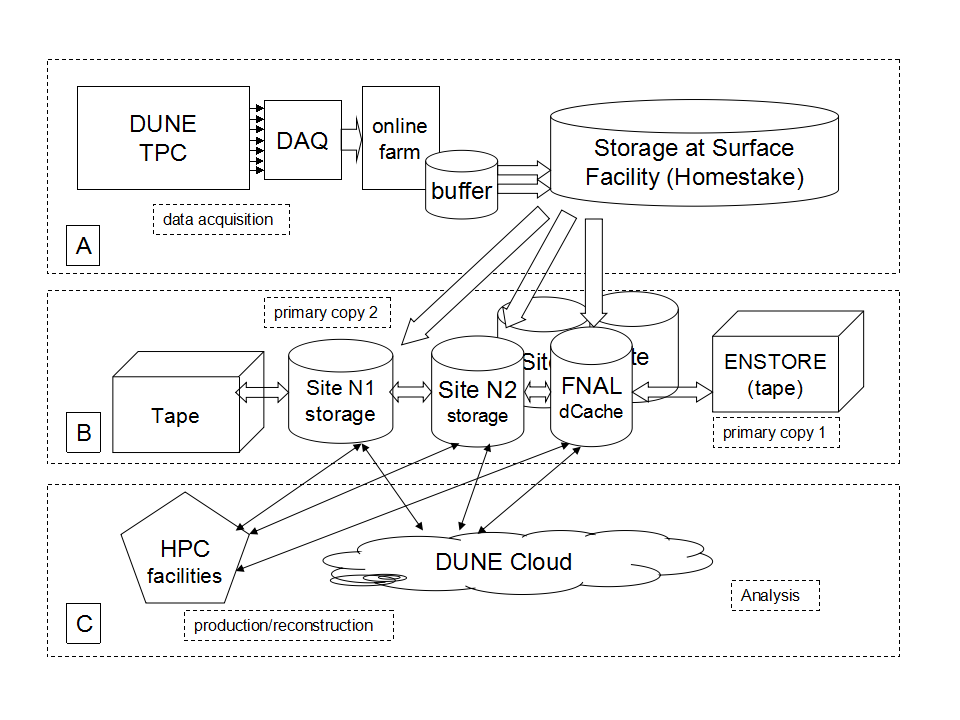
\includegraphics[width=\textwidth]{DUNEdataflow.png}
\caption{Dataflow in DUNE (concept).}
\label{fig:DUNEdataflow}
\end{figure}